\subsection{Phénomène}

\begin{definition}
On appelle \tdef{phénomène d'interférences} la superposition de plusieurs \imp{\abr{ops} synchrones}.

\begin{figure}[H]
\begin{center}
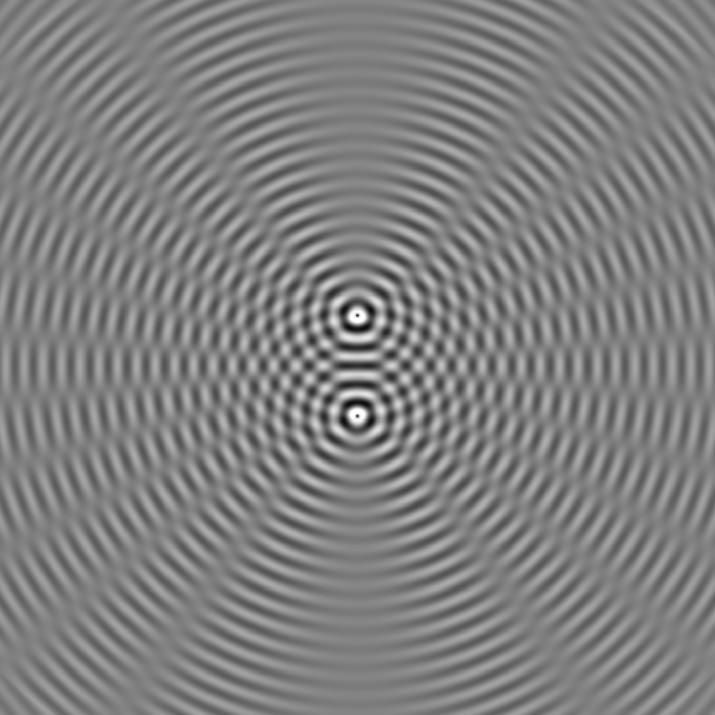
\includegraphics[width=3.5cm]{01_signaux_harmoniques_propagation/interferences.png}

\captionsetup{labelformat=empty}
\caption{Figure d'interférences à la surface d'une cuve à ondes}
\end{center}
\end{figure}
\end{definition}

\begin{propriete}
Soit $s_1(\point{M}, t)$ et $s_2(\point{M}, t)$ deux \imp{\abr{ops} synchrones} de pulsation $\omega$ :
\[\begin{cases}
s_1(\point{M}, t) = A_1 \cos(\omega t + \varphi_1(\point{M}))\\
s_2(\point{M}, t) = A_2 \cos(\omega t + \varphi_2(\point{M}))
\end{cases}\]
Alors l'onde  $s(\point{M}, t)$ résultant de la superposition de $s_1(\point{M}, t)$ et $s_2(\point{M}, t)$ a en tout point $\point{M}$ la forme d'un signal sinusoïdal de même pulsation $\omega$ :
\[s(\point{M}, t) = s_1(\point{M}, t) + s_2(\point{M}, t) = A_r(\point{M}) \cos(\omega t + \varphi_r(\point{M}))\]
\end{propriete}



\subsection{Représentation de Fresnel}

\begin{definition}
La \tdef{représentation de Fresnel} d'un \imp{signal sinusoïdal} $A \cos(\omega t + \varphi)$ est le vecteur du plan complexe d'amplitude $A$ et faisant un angle $\varphi$ avec l'axe des réels :

\begin{figure}[H]
\begin{center}
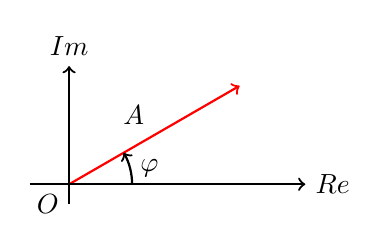
\begin{tikzpicture}[thick]
\coordinate (O) at (0,0);

\draw [red, ->] (O) -- node [above left, black] {$A$} (30:2.5cm);
\draw [->] (O) +(0.8,0) arc (0:30:0.8) node [midway, right] {$\varphi$};

\draw [->] (O) +(-0.5,0) -- +(3,0) node [right] {$\mathfrak{Re}$};
\draw [->] (O) +(0,-0.25) -- +(0,1.5) node [above] {$\mathfrak{Im}$};

\node [below left] at (O) {$\point{O}$};
\end{tikzpicture}
\end{center}
\end{figure}
\end{definition}

\begin{propriete}[admis]
La représentation de Fresnel de la somme de deux \imp{signaux sinusoïdaux synchrones} est la somme des leurs.
\end{propriete}

\begin{propriete}
En reprenant les notations précédentes, on a :
\[A_r(\point{M})^2 = {A_1}^2 + {A_2}^2 + 2 A_1 A_2 \cos \Delta\varphi(\point{M})\]

\begin{figure}[H]
\begin{center}
\begin{tikzpicture}[thick]
\coordinate (O) at (0,0);
\coordinate (Q) at ($ (O) + (20:3cm) $);
\coordinate (P) at ($ (Q) + (75:3cm) $);

\draw [red, ->] (O)  -- node [above left, black] {$A_r(\point{M})$} (P);
\draw [blue, ->] (O) -- node [above left, black] {$A_1$} (Q);
\draw [blue, ->] (Q) -- node [left, black] {$A_2$} (P);

\draw [->] (O) +(1,0) arc (0:20:1)  node [midway, right] {$\varphi_1$};
\draw [->] (Q) +(1,0) arc (0:75:1);
\path      (Q) +(1,0) arc (0:20:1) node [midway, right] {$\varphi_2$};
\draw [->] (Q) +($ 1.2*({cos(20)},{sin(20)}) $) arc (20:75:1.2) node [midway, above right] {$\Delta\varphi(\point{M})$};

\draw [dashed] (Q) -- +(3,0);
\draw [dashed] (Q) -- +(Q);

\draw [->] (O) +(-1,0) -- +(6.5,0) node [right] {$\mathfrak{Re}$};
\draw [->] (O) +(0,-0.5) -- +(0,4) node [above] {$\mathfrak{Im}$};

\node [below left] at (O) {$\point{O}$};
\end{tikzpicture}
\end{center}
\end{figure}

\end{propriete}



\subsection{Cas particuliers}

\begin{propriete}
Toujours avec les notations précédentes, pour $\point{M}$ un point quelconque de l'espace, si les deux ondes $s_1(\point{M}, t)$ et $s_2(\point{M}, t)$ : 

\begin{itemize}
\item arrivent \imp{en phase} en $\point{M}$, c'est-à-dire si $\Delta\varphi(\point{M}) = 0$, alors l'amplitude résultante $A_r(\point{M})$ est maximale et vaut :
\[A_r(\point{M}) = A_1 + A_2\]
On parle alors d'\tdef{intérférences constructives};

\item arrivent \imp{en  opposition de phase} en $\point{M}$, c'est-à-dire si $\Delta\varphi(\point{M}) = \pi$, alors $A_r(\point{M})$ est minimale et vaut :
\[A_r(\point{M}) = \abs{A_1 - A_2}\]
On parle d'\tdef{intérférences destructives}.
\end{itemize}
\end{propriete}